\renewcommand*{\arraystretch}{1.1}

\noindent\begin{tabularx}{17cm}{|p{1.95cm}|X|}
	\hline
	workload    & Interactive / short \\ \hline
%
	query       & 5 \\ \hline
%
	title       & Message Creator \\ \hline
%
    pattern     & \hfill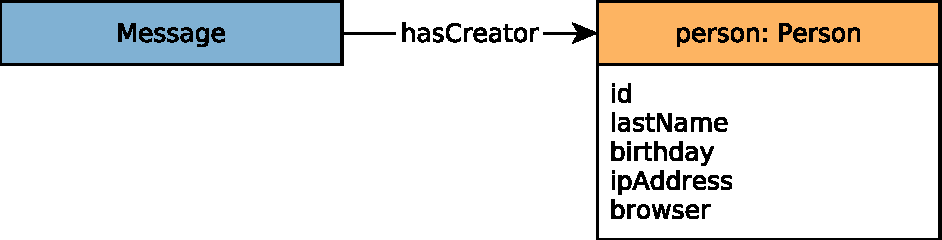
\includegraphics[scale=\patternscale,margin=0cm .2cm]{patterns/interactive-short-read-05}\hfill\vadjust{} \\ \hline
%
	description & Given a Message, retrieve its author.
 \\ \hline
%
	
%
	parameters  &
	\vspace{1.1ex}{\begin{tabularx}{14.2cm}{|c|M|m{2cm}|Y|} \hline
	\cellcolor{parameter} \color{white} $\mathsf{1}$ & \varname{Message.id} & \cellcolor{gray!20} \vartype{ID} &  \\ \hline
	\end{tabularx}}\vspace{1.1ex} \\ \hline
%
	
	result      &
	\vspace{1.1ex}{\begin{tabularx}{14.2cm}{|c|M|m{2cm}|c|Y|} \hline
	\cellcolor{result} \color{white} $\mathsf{1}$ & \varname{Message-hasCreator->Person.id} & \cellcolor{gray!20} \vartype{ID} &
	    \texttt{R} &
	     \\ \hline
	\cellcolor{result} \color{white} $\mathsf{2}$ & \varname{Message-hasCreator->Person.firstName} & \cellcolor{gray!20} \vartype{String} &
	    \texttt{R} &
	     \\ \hline
	\cellcolor{result} \color{white} $\mathsf{3}$ & \varname{Message-hasCreator->Person.lastName} & \cellcolor{gray!20} \vartype{String} &
	    \texttt{R} &
	     \\ \hline
	\end{tabularx}}\vspace{1.1ex} \\ \hline
	
%
	%
	%
	%
\end{tabularx}
\vspace{2ex}